\documentclass[12pt]{report}
\usepackage{amsmath}
\usepackage{ragged2e}
\usepackage{graphicx}
\usepackage{multirow}
\usepackage[absolute,overlay]{textpos}
\graphicspath{ {./img/} }
\setlength\parindent{0pt}

\newcommand{\thn}{\textsuperscript{th}}

\newcommand{\twopartdef}[4]
{
	\left\{
	\begin{array}{ll}
		#1 & \mbox{} #2 \\
		#3 & \mbox{} #4
	\end{array}
	\right.
}

\newcommand{\threepartdef}[6]
{
	\left\{
	\begin{array}{lll}
		#1 & \mbox{} #2 \\
		#3 & \mbox{} #4 \\
		#5 & \mbox{} #6
	\end{array}
	\right.
}

\begin{document}

\Large
\centering
AMS310 Homework 3

\justify
\normalsize

Kuba Gasiorowski\\
ID: 109776237\\

\noindent \textbf{1a.} In order to prove $f(x)$ is a pdf we must show the following:
\begin{enumerate}
	\item $\forall x, f(x) \geq 0$
	\item $\int_{-\infty}^{\infty} f(x)dx = 1$
\end{enumerate}

\noindent (1) is obvious, since it is given that $ f(x) = \frac{1}{3}, 0 < x < 3 $, and we can assume $f(x) = 0, x \leq 0 \;\text{and}\; x \geq 3$. Thus $\forall x, f(x) \geq 0$.\\

\noindent (2) can be found by taking the following integral: 
\begin{align*}
\int_{0}^{3}\frac{1}{3}dx &= 1\\
\frac{1}{3}\int_{0}^{3}1dx &= 1\\
\frac{1}{3}\left[x\right]_0^3 &= 1\\
\frac{1}{3}(3 - 0) &= 1\\
1 &= 1
\end{align*}

\noindent Thus $f(x)$ is a pdf. \\

\pagebreak

\noindent \textbf{b.} To find the mean ($\mu$) of $f(x)$:

\begin{align*}
\mu &= \int_{-\infty}^{\infty} xf(x)dx \\
\mu &= \int_0^3 x\frac{1}{3}dx \\
\mu &= \frac{1}{3}\int_0^3 xdx \\
\mu &= \frac{1}{3} \cdot \left[\frac{x^2}{2}\right]_0^3 \\
\mu &= \frac{1}{3} \cdot \left(\frac{3^2}{2} - \frac{0^2}{2}\right)\\
\mu &= \boxed{\frac{9}{6} = 1.5}
\end{align*}

\noindent And then the variance ($\sigma$):

\begin{align*}
\sigma^2 &= \int_{-\infty}^{\infty} x^2f(x)dx - \mu^2\\
\sigma^2 &= \int_{0}^{3} \frac{1}{3}x^2dx - 2.25\\
\sigma^2 &= \frac{1}{3}\int_{0}^{3}x^2dx - 2.25\\
\sigma^2 &= \frac{1}{3} \cdot \left[ \frac{x^3}{3} \right]_0^3 - 2.25\\
\sigma^2 &= \frac{1}{3} \cdot 9 - 2.25\\
\sigma^2 &= \boxed{0.75}\\
\end{align*}

\pagebreak

\noindent \textbf{e.} Find $P(\frac{1}{2} < X < \frac{5}{2})$:
\begin{align*}
(\frac{1}{2} < X < \frac{5}{2}) &= \int_{\frac{1}{2}}^{\frac{5}{2}}\frac{1}{3}dx\\
&= \frac{1}{3}\int_{\frac{1}{2}}^{\frac{5}{2}}1dx\\
&= \frac{1}{3}\left[x\right]_{\frac{1}{2}}^{\frac{5}{2}}\\
&= \frac{1}{3}\left(\frac{5}{2} - \frac{1}{2}\right)\\
&= \boxed{\frac{2}{3} \approx .66\overline{6}}\\
\end{align*}

\noindent \textbf{f.} Find $P(X > 1)$:
\begin{align*}
P(X > 1) &= \int_1^{\infty}f(x)dx\\
&= \int_{1}^{3}\frac{1}{3}dx\\
&= \frac{1}{3}\int_{1}^{3}1dx\\
&= \frac{1}{3}\left[x\right]_1^3\\
&= \frac{1}{3}(3-1)\\
&= \boxed{\frac{2}{3} \approx .66\overline{6}}
\end{align*}

\pagebreak

\noindent \textbf{g.} Find the 40\thn percentile.

\begin{align*}
\int_{0}^{x_{0.4}}f(x)dx &= 0.4\\
\int_{0}^{x_{0.4}}\frac{1}{3}dx &= 0.4\\
\frac{1}{3}\int_{0}^{x_{0.4}}1dx &= 0.4\\
\frac{1}{3}[x]_0^{x_{0.4}} &= 0.4\\
\frac{1}{3}x_{0.4} &= 0.4\\
x_{0.4} &= \boxed{1.2}
\end{align*}

\noindent \textbf{2a.} Given $N(90, 225)$, find $P(X > 80)$.\\\\
\noindent We have $\mu = 90$, $\sigma^2=225 \Rightarrow \sigma = 15$, and $x = 80$.
\begin{align*}
z &= \frac{x - \mu}{\sigma}\\
z &= \frac{80 - 90}{15}\\
z &\approx -.67
\end{align*}

\noindent Then using the normal tables, we get $.2514$ as the area underneath the curve to the left of $z = -0.66$. Since we want to know the area to the right, we subtract that from 1 and get $\boxed{0.7486} = 74.86\%$ as the answer.\\

\noindent \textbf{b.} We use the above formula, except solving for x for the z-score that corresponds to 75\%. The closest z-score to .75 is 0.68. Then we have:
\begin{align*}
\frac{x-\mu}{\sigma} &= z\\
x &= z\sigma + \mu\\
x &= 0.68 \cdot 15 + 90\\
x &= 100.2
\end{align*}

\noindent Thus the weight that separates the top 25\% of the male sheep is approximately \boxed{100.2 \text{ pounds}}.\\

\noindent \textbf{3a.} We have $N(\mu = 115000, \sigma^2 = 10000^2)$. Find $P(X > 130000)$. \\
\begin{align*}
z &= \frac{x - \mu}{\sigma}\\
z &= \frac{130000 - 115000}{10000}\\
z &= 1.5
\end{align*}

\noindent Then using the normal tables to convert the z-score to a percent, we obtain 0.9332. Then we find 1 - 0.9332 and get 0.0668 or \boxed{6.68\%} of timing belts last 130k miles or more.\\

\noindent \textbf{b.} Find $P(X < 100000)$.

\begin{align*}
z &= \frac{x-\mu}{\sigma}\\
z &= \frac{100000 - 115000}{10000}\\
z &= -1.5
\end{align*}

\noindent Using the normal tables: $z = -1.5 \Rightarrow 0.0668$. Thus the chance of a timing belt failing at less than 100k is about 6.68\%.\\

\noindent \textbf{c.} First we find the z-score that corresponds to .75, which is $\approx 0.68$. Then we plug and chug.
\begin{align*}
x &= z\sigma + \mu\\
x &= 0.86 \cdot 10000 + 115000\\
x &= \boxed{121800 \text{ miles}}
\end{align*}

\noindent \textbf{4.} First, we have $\lambda = 30$ and $P(X) \Rightarrow F(x) = 1- e^{-\frac{x}{\lambda}}$
\begin{align*}
P(X < 25) &= 1-e^{-\frac{25}{30}}\\
&= 1-e^{-\frac{5}{6}}\\
&\approx 1-0.4346\\
&\boxed{\approx 0.5654}
\end{align*}

\begin{align*}
P(X > 35) &= 1 - P(X < 35)\\
&= 1 - \left(1 - e^{-\frac{35}{30}}\right)\\
&= e^{-\frac{7}{6}}\\
&\approx \boxed{0.3114 \approx 31.14\%}
\end{align*}

\begin{align*}
P(25 < X < 35) &= P(X < 35) - P(X < 25)\\
&= (1-P(X > 35)) - P(X < 25)\\
&= (1 - 0.3012)-0.5654\\
&= \boxed{0.1334 = 13.34\%}
\end{align*}

\noindent \textbf{b.}
\begin{align*}
F(x) &= \frac{1}{2}, \; (\lambda = 30)\\
1-e^{-\frac{x}{30}} &= \frac{1}{2}\\
e^{-\frac{x}{30}} &= \frac{1}{2} \\
-\frac{x}{30} &= \ln{\frac{1}{2}}\\
x &= -30\ln{\frac{1}{2}}\\
x &\approx \boxed{20.79}
\end{align*}

\pagebreak

\noindent \textbf{5a.} Since we must satisfy \\

$$ \int_{-\infty}^{\infty} f(x)dx = 1 \Rightarrow \int_{40}^{100}f(x)dx = 1$$\\
\noindent It's easy to see that $f(x) = \frac{1}{60}$ satisfies the above. So we can draw the pdf as follows:\\

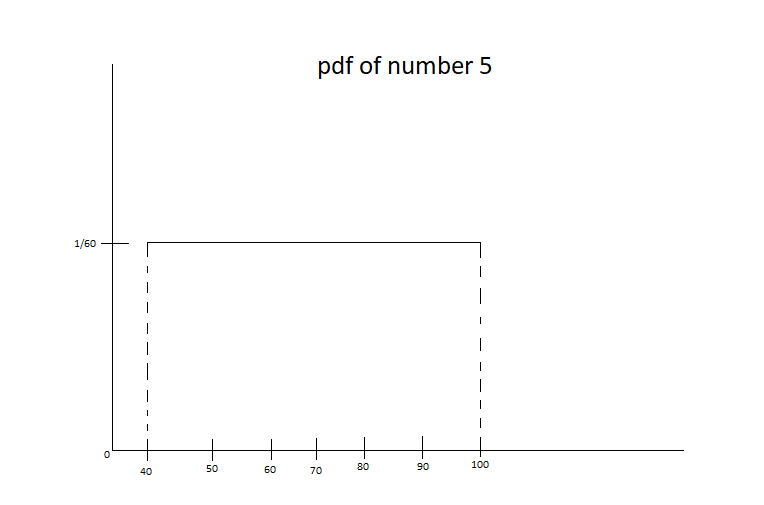
\includegraphics[scale=.7]{hw3_5}

\noindent So in summary, we have:\\

\centering
$f(x) = \twopartdef{\frac{1}{60}}{40 \leq x \leq 100}{0}{\text{otherwise}}$\\
\bigskip
\noindent And\\
\bigskip
$F(x) = \threepartdef{0}{x < 40}{\frac{x}{60}}{40 \leq x \leq 100}{1}{x > 100}$\\

\justify

\pagebreak
\noindent Now we can easily calculate $P(50 < X < 70)$:
\begin{align*}
P(50 < X < 70) &= P(70) - P(50)\\
&= F(70) - F(50)\\
&= \frac{70}{60} - \frac{50}{60}\\
&= \boxed{\frac{1}{3} \approx 33.3\overline{3}\%}
\end{align*}

\noindent And it can be visualized like so:

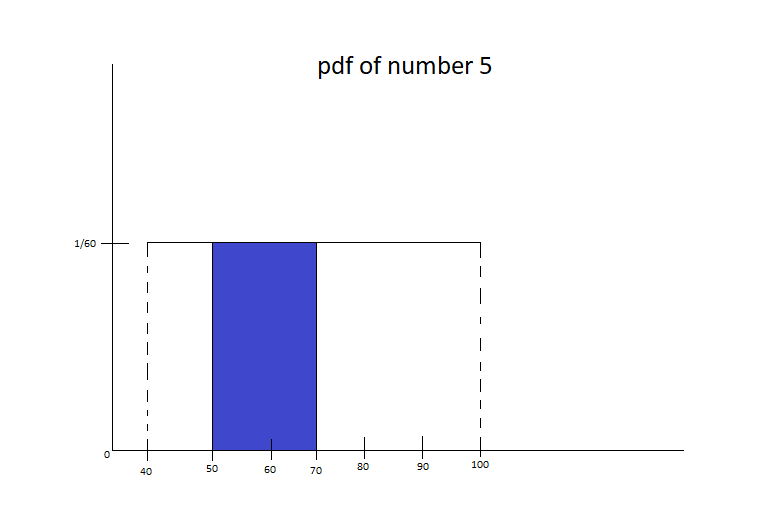
\includegraphics[scale = .7]{hw3_5a}

\pagebreak

\noindent \textbf{b.}

\begin{align*}
P(X < 75) &= F(75) - F(40)\\
&= \frac{75}{60} - \frac{40}{60}\\
&= \boxed{\frac{35}{60} = \frac{7}{12} \approx .5833\overline{3}}
\end{align*}
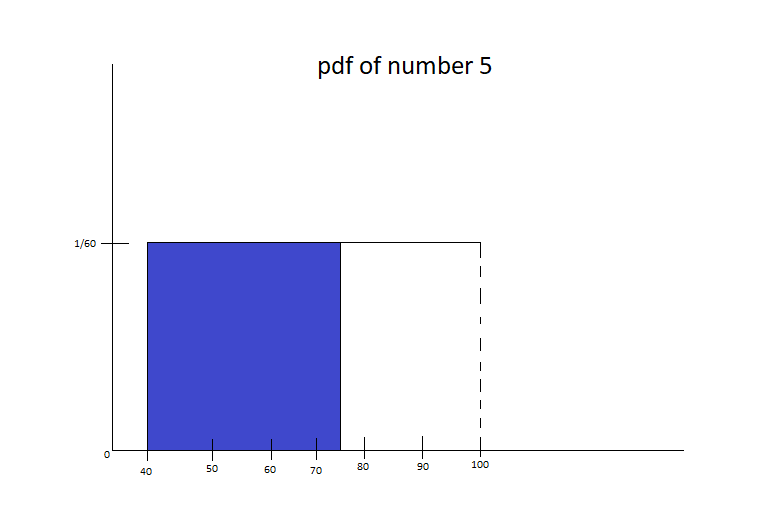
\includegraphics[scale = .7]{hw3_5b}\\
\pagebreak

\noindent \textbf{c.} 
\begin{align*}
P(X > 90) &= P(100) - P(90)\\
&= F(100) - F(90)\\
&= \frac{100}{60} - \frac{90}{60}\\
&= \frac{10}{60} \\
&= \boxed{\frac{1}{6} \approx 0.166\overline{6}}
\end{align*}

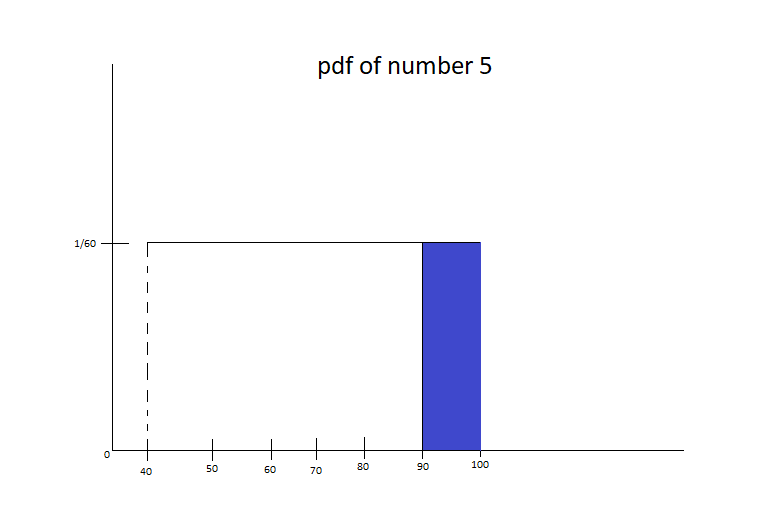
\includegraphics[scale = .7]{hw3_5c}

\pagebreak
\noindent \textbf{d.} 
\begin{align*}
P(40 < X < x) &= 0.95\\
P(x) - P(40) &= 0.95\\
F(x) - F(40) &= 0.95\\
\frac{x-40}{60} &= 0.95\\
x &= \boxed{97}
\end{align*}

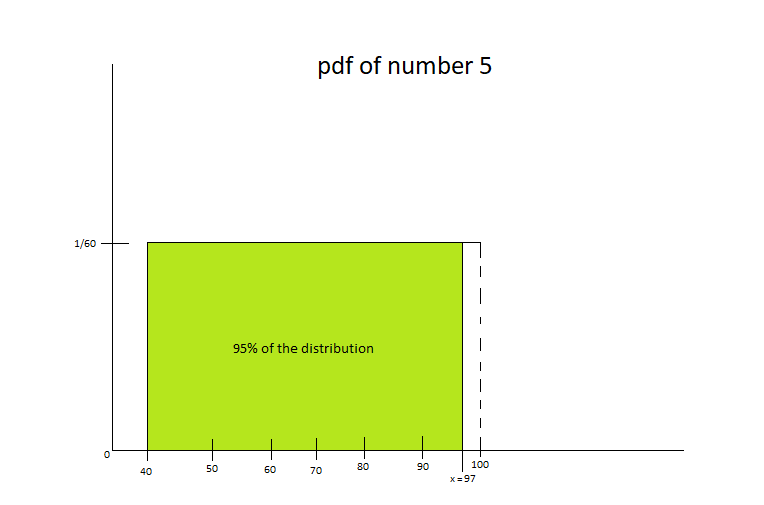
\includegraphics[scale = 0.7]{hw3_5d}\\

\noindent \textbf{6a.} 
\begin{verbatim}
> pexp(.65, 1/.75)
[1] 0.5796496
\end{verbatim}

\noindent \textbf{b.}
\begin{verbatim}
> lambda <- .75
> pexp(2, 1/lambda)-pexp(.75, 1/lambda)
[1] 0.298396
\end{verbatim}

\pagebreak
\noindent \textbf{c.} 
\begin{verbatim}
> qexp(.95, 1/lambda)
[1] 2.246799
\end{verbatim}

\noindent \textbf{7a.} $\mu = E(X) = \alpha\beta = (3)(5) = \boxed{15}$\\
\noindent \textbf{b.} $\sigma^2 = \alpha\beta^2 \Rightarrow \sigma = \sqrt{\alpha\beta^2} = \sqrt{(3)(5)^2} = 5\sqrt{3} \approx \boxed{8.660}$\\
\noindent \textbf{c.} 
\begin{verbatim}
> pgamma(4.5, 3, 1/5)
[1] 0.06285693
\end{verbatim}

\noindent \textbf{d.}
\begin{verbatim}
> pgamma(5, 3, 1/5) - pgamma(2, 3, 1/5)
[1] 0.07237507
\end{verbatim}

\noindent \textbf{8a.} The pdf will look like this:\\ 
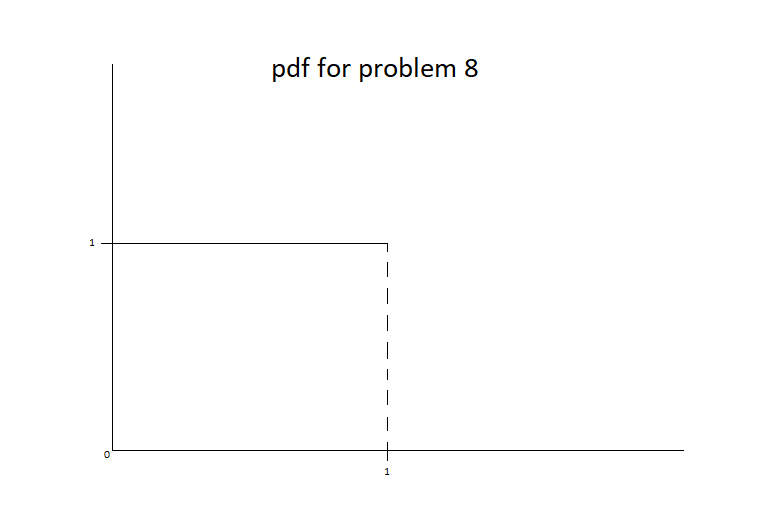
\includegraphics[scale = .7]{hw3_8}

\noindent \textbf{b.} This is also known as a uniform(0,1) distribution.

\noindent \textbf{c.} The cdf is just the area function of the pdf. So it'll look like the following:\\
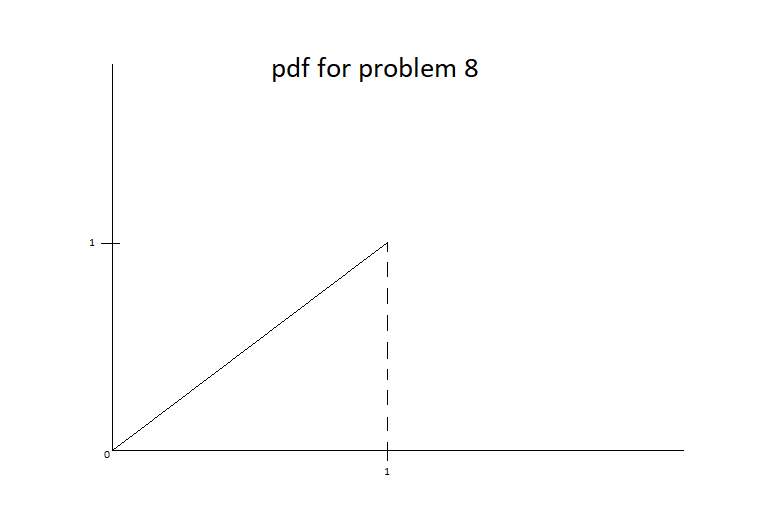
\includegraphics[scale = 1]{hw3_8c}

\noindent \textbf{9a.} $\mu = np = 1000(0.15) = 150$\\
$\sigma = \sqrt{np(1-p)} = \sqrt{1000(0.15)(0.85)} \approx11.291$
\begin{align*}
P(X < 125) &= P\left(Z \leq \frac{(X-0.5) - \mu}{\sigma}\right)\\
&= P\left(Z \leq \frac{124.5 - 150}{11.291}\right)\\
&= P(Z \leq -2.26)\\
&= \boxed{.01539}
\end{align*}
\noindent \textbf{b.} 
\begin{align*}
P(X \geq 150) &= P\left(Z \geq \frac{(X - 0.5)-\mu}{\sigma}\right)\\
&= P\left(Z \geq \frac{150.5 - 150}{11.291}\right)\\
&= P(Z \geq 0.0442)\\
&= 1 - 0.5160 = \boxed{0.4840}
\end{align*}
\noindent \textbf{c.} 
\begin{verbatim}
> pbinom(125, 1000, 0.15)
[1] 0.01349891
> 1 - pbinom(150, 1000, 0.15)
[1] 0.4782311
\end{verbatim}

\noindent \textbf{10a.}

\begin{textblock*}{1cm}(3.25cm, 9cm)
	X
\end{textblock*}

\begin{tabular}{|p{2cm}||p{2cm}|p{2cm}|p{2cm}|p{2cm}|}
	\multicolumn{5}{c}{Y} \\
	\hline
	f(x,y) & +15\% & +5\% & 0\% & -5\%\\
	\hline
	\hline
	+30\% & 0.1 & 0.0625 & 0.05 & 0.0375\\
	\hline
	+10\% & 0.12 & 0.075 & 0.06 & 0.045\\
	\hline
	+5\% & 0.08 & 0.05 & 0.04 & 0.03\\
	\hline
	-10\% & 0.1 & 0.0625 & 0.05 & 0.0375\\
	\hline
\end{tabular}
\bigskip\\
\noindent \textbf{b.} To find the chance that you will lose money if you invest in X, you have to add up all the values in the table such that X has a negative return: 
\begin{align*}
P(X\text{ loses money}) &= 0.1 + 0.0625 + 0.05 + 0.0375\\
&= \boxed{0.25}
\end{align*}
\noindent We do the same for $Y$:
\begin{align*}
P(Y\text{ loses money}) &= 0.0375 + 0.045 + 0.03 + 0.0375\\
&= \boxed{0.15}
\end{align*}
\noindent \boxed{\text{Thus investing in $Y$ is a safer bet.}}
\\\\
\noindent \textbf{c.} 

\begin{textblock*}{1cm}(2.75cm, 18.75cm)
	X\\
	(\$10,000)
\end{textblock*}

\begin{tabular}{|p{3cm}||p{2.8cm}|p{2.7cm}|p{2.5cm}|p{2.5cm}|}
	\multicolumn{5}{c}{Y (\$30,000)} \\
	\hline
	f(x,y) & +15\% $\rightarrow$ \$4500& +5\% $\rightarrow$ \$1500& 0\% $\rightarrow$ \$0& -5\% $\rightarrow$ -\$1500\\
	\hline
	\hline
	+30\%  $\rightarrow$ \$3000& \$7500 & \$4500 & \$3000 & \$1500\\
	\hline
	+10\% $\rightarrow$ \$1000& \$5500 & \$2500 & \$1000 & -\$500\\
	\hline
	+5\% $\rightarrow$ \$500& \$5000 & \$2000 & \$500 & -\$1000\\
	\hline
	-10\% $\rightarrow$ -\$1000& \$3500 & \$500 & -\$1000 & -\$2500\\
	\hline
\end{tabular}
\bigskip\\
\noindent \textbf{d.} In order to find the probability of a loss, we just add up all the probabilities where the overall return is negative:
\begin{align*}
P(f(x,y) < 0) &= 0.045 + 0.03 + 0.05 + 0.0375\\
&= \boxed{0.1625}
\end{align*}

\pagebreak
\noindent \textbf{11a.} 
\begin{align*}
f_1(x) &= \int_0^xf(x,y)dx\\
&= \int_{0}^x15xy^2dy\\
&= \left[5xy^3\right]_0^x\\
&= \boxed{5x^4}
\end{align*}

\noindent \textbf{b.}
\begin{align*}
f_2(y|x) &= \frac{f(x,y)}{f_1(x)}\\
&= \frac{15xy^2}{5x^4}\\
&= \boxed{\frac{3y^2}{x^3}}
\end{align*}
\noindent \textbf{c.}
\begin{align*}
\forall x > \frac{1}{3}, \;P(Y > \frac{1}{3}|X = x) &= 1 - \int_0^\frac{1}{3} f_2(y|x)dy\\
&= 1- \int_0^\frac{1}{3} \frac{3y^2}{x^3}dy\\
&= 1-\left[\frac{y^3}{x^3}\right]_0^\frac{1}{3}\\
&= \boxed{1 - \left(\frac{1}{27x^3}\right)}
\end{align*}

\noindent \textbf{d.} They cannot possibly be independent because $f_2(y|x) = \frac{3y^2}{x^3}$ (from part b) includes $x$. \\
\pagebreak

\noindent \textbf{12a.} 
\begin{align*}
f(x,y) &= f_1(x)f_2(y) \\
&= \left(\frac{1}{2}e^{-\frac{x}{2}}\right)\left(\frac{1}{5}e^{-\frac{y}{5}}\right)\\
&= \boxed{\frac{1}{10}e^{\left(-\frac{x}{2} - \frac{y}{5}\right)}}
\end{align*}

\noindent \textbf{b.}
\begin{align*}
f_2(y|x) &= f_2(y)\\
&= \boxed{\frac{1}{5}e^{-\frac{y}{5}}, \; y \geq 0}
\end{align*}

\noindent \textbf{c.} 
\begin{align*}
P(X > 3, Y > 6) &= P(X > 3)P(Y > 6)\\
&= [1 - F_1(3)][1 - F_2(6)]\\
&= \left[1 - \left(1 - e^{-\frac{3}{2}}\right)\right]\left[1 - \left(1 - e^{-\frac{6}{5}}\right)\right]\\
&= \left(e^{-\frac{3}{2}}\right)\left(e^{-\frac{6}{5}}\right)\\
&\approx \boxed{0.0672}
\end{align*}

\noindent \textbf{d.} 
\begin{align*}
P(X > 3|Y = 6) &= P(X > 3)\\
&= 1 - F_1(3)\\
&= 1 - (1 - e^{-\frac{3}{2}})\\
&= e^{-\frac{3}{2}}\\
&\approx \boxed{0.223} 
\end{align*}

\pagebreak
\noindent \textbf{13a.} 
\begin{align*}
P(X+Y \leq 4) &= f(1,1) + f(1,2) + f(1,3) + f(2,1) + f(3,1) + f(2,2)\\
&= 0.1 + 0.05 + 0.15 + 0.1 + 0.15 + 0.05\\
&= \boxed{0.6} 
\end{align*}

\noindent \textbf{b.}
\begin{align*}
f_1(1) &= 0.1 + 0.05 + 0.15 = 0.3\\
f_1(2) &= 0.1 + 0.05 + 0.1 = 0.25\\
f_1(3) &= 0.15 + 0.2 + 0.1 = 0.45\\\\
f_2(1) &= 0.1 + 0.1 + 0.15 = 0.35\\
f_2(2) &= 0.05 + 0.05 + 0.2 = 0.3\\
f_2(3) &= 0.15 + 0.1 + 0.1 = 0.35 
\end{align*}

\noindent \textbf{c.}
\begin{align*}
P(X < 2 | Y = 2) &= P(X = 1 | Y = 2)\\
&= \frac{f(1,2)}{f_2(2)}\\
&= \frac{0.05}{0.3}\\
&= \boxed{\frac{1}{6}}
\end{align*}

\noindent \textbf{d.} X and Y cannot possibly be independent because $f_1(1|2) \neq f_1(1)$.\\
\noindent \textbf{e.} 
\begin{align*}
E(X) &= \sum xf_1(x) = 1 \cdot 0.3 + 2 \cdot 0.25 + 3 \cdot 0.45 = \boxed{2.15}\\
E(Y) &= \sum yf_2(y) = 1 \cdot 0.35 + 2 \cdot 0.3 + 3 \cdot 0.35 = \boxed{2}\\ 
\end{align*}

\pagebreak
\noindent \textbf{f.} 
\begin{align*}
\text{Var}(X) &= E\left[\left(X - \mu_X\right)^2\right] = \sum\left(x - \mu_X\right)^2f_1(x)\\
&= 0.3(1 - 2.15)^2 + 0.25(2 - 2.15)^2 + 0.45(3 - 2.15)^2\\
&= \boxed{0.7275}\\\\
\text{Var}(Y) &= E\left[\left(Y - \mu_Y\right)^2\right] = \sum\left(y - \mu_Y\right)^2f_2(y)\\
&= 0.35(1 - 2)^2 + 0.3(2-2)^2 + 0.35(3-2)^2\\
&= \boxed{0.7}
\end{align*}

\noindent \textbf{g.}
\begin{align*}
E(X, Y) &= 1(0.1) + 2(0.05 + 0.1) + 3(0.15 + 0.15) + 4(0.05) + 6(0.2 + 0.1) + 9(0.1)\\
&= 4.2\\\\
Cov(X, Y) &= E(X, Y) - E(X)E(Y)\\
&= 4.2 - 2 \cdot 2.15\\
&= -0.1\\\\
\text{correlation coefficient} &= \frac{Cov(X, Y)}{\sigma_x\sigma_y} = \frac{-0.1}{\sqrt{(0.7275)(0.7)}} = \boxed{0.1401}
\end{align*}

\pagebreak
\noindent \textbf{14a.} 
\begin{align*}
\begin{aligned}[c]
f(x) &= \int_{0}^{1}f(x, y)dy\\
&= \int_0^1\frac{3}{4}\left(x^2 + 3y^2\right)dy\\
&= \left[\frac{3}{4}x^2y+\frac{3}{4}y^3\right]_0^1\\
&= \boxed{\frac{3}{4}x^2+\frac{3}{4}}
\end{aligned}
\begin{aligned}[c]
f(y) &= \int_{0}^{1}f(x, y)dx\\
&= \int_0^1\frac{3}{4}\left(x^2 + 3y^2\right)dx\\
&= \left[\frac{1}{4}x^3 + \frac{9}{4}y^2x\right]_0^1\\
&= \boxed{\frac{9}{4}y^2 + \frac{1}{4}}
\end{aligned}
\end{align*}

\noindent \textbf{b.}
\begin{align*}
\begin{aligned}[c]
F(x) &= \int_{0}^{x}f(x)dx\\
&= \int_{0}^{x}\frac{3}{4}x^2 + \frac{3}{4}dx\\
&= \left[\frac{1}{4}x^3 + \frac{3}{4}x\right]_0^x\\
&= \boxed{\frac{1}{4}x^3+\frac{3}{4}} 
\end{aligned}
\begin{aligned}[c]
F(y) &= \int_{0}^{y}f(y)dy\\
&= \int_{0}^{y}\frac{9}{4}y^2 + \frac{1}{4}\\
&= \left[\frac{3}{4}y^3+\frac{1}{4}y\right]_0^y\\
&= \boxed{\frac{3}{4}y^3+\frac{1}{4}y}
\end{aligned}
\end{align*}

\noindent \textbf{c.}
\begin{align*}
f_1(x|y) &= \twopartdef{\frac{f(x,y)}{f_2(y )} = \frac{3x^2 + 9y^2}{1+9y^2}}{0 < x < 1, 0 < y < 1}{0}{otherwise}\\
f_2(y|x &= \twopartdef{\frac{f(x,y)}{f_1(x)} = \frac{x^2 + 3y^2}{x^2+1}}{0 < x < 1, 0 < y < 1}{0}{otherwise}
\end{align*}

\noindent \textbf{d.}
\begin{align*}
E(x) &= \int_0^1x\left(\frac{3}{4}x^2 + \frac{3}{4}\right)dx = \left[\frac{3}{16}x^4 + \frac{3}{8}x^2\right]_0^1 = \boxed{\frac{9}{16}}\\
E(y) &= \int_0^1y\left(\frac{1}{4} + \frac{9}{4}y^2\right)dx = \left[\frac{1}{8}y^2 + \frac{9}{16}y^4\right]_0^1 = \boxed{\frac{11}{16}}\\
\end{align*}

\noindent \textbf{e.}
\begin{align*}
\text{Var}(x) &= E(x^2) - E(x)^2 = \frac{2}{5} - \frac{81}{256} = \boxed{0.084}	\\
\text{Var}(y) &= E(y^2) - E(y)^2 = \frac{8}{15} - \frac{121}{256} = \boxed{0.061}
\end{align*}

\noindent \textbf{f.}
\begin{align*}
E(x,y) &= \int_{-\infty}^{\infty}xyf(x,y)dxdy\\
&= \frac{3}{4}\int_{0}^{1}\int_{0}^{1}xy(x^2 + 3y^2)dxdy\\
&= \frac{3}{4}\int_{0}^{1}\int_0^1(x^3y + 3xy^3)dxdy\\
&= \frac{3}{4}\int_0^1\left[\frac{x^4y}{4} + \frac{3x^2y^3}{2}\right]_0^1dy\\
&= \frac{3}{4}\int_{0}^{1}\left(\frac{y}{4} + \frac{3y^3}{1}\right)dy\\
&= \frac{3}{4}\left[\frac{y^2}{8} + \frac{3y^4}{8}\right]_0^1\\
&= \frac{3}{4}\left(\frac{1}{8} + \frac{3}{8}\right) = \boxed{\frac{3}{8}}
\end{align*}

$$ Cov(X, Y) = E(X,Y) - E(X)E(Y) = \frac{3}{8} - \frac{9}{16} \cdot \frac{11}{16} = \boxed{\frac{-3}{256}}$$

\pagebreak
\noindent \textbf{g.} Find $P(Y < \frac{1}{3}|X < \frac{1}{3})$:\\

We have $P(Y < \frac{1}{3}|X < \frac{1}{3}) = \frac{P(Y < \frac{1}{3}, X < \frac{1}{3})}{P(X < \frac{1}{3})}$.

\begin{align*}
P\left(Y < \frac{1}{3}, X < \frac{1}{3}\right) &= \int_{0}^{\frac{1}{3}}\int_0^{\frac{1}{3}}\frac{3}{4}(x^2+3y^2)dxdy\\
&= \int_0^{\frac{1}{3}}\frac{3}{4}\left[\frac{x^2}{3} + 3xy^2\right]_0^{\frac{1}{3}}dy\\
&= \int_{0}^{\frac{1}{3}}\left(\frac{1}{108} + \frac{1}{4}y^2\right)dy\\
&= \left[\frac{y}{108} + \frac{y^3}{12}\right]_0^{\frac{1}{3}}\\
&= \boxed{\frac{1}{162}}\\\\
P\left(X < \frac{1}{3}\right) &= \int_0^\frac{1}{3}\frac{3}{4}(x^2+1)dx\\
&= \left[\frac{1}{4}x^3 + \frac{3}{4}x\right]_0^\frac{1}{3}\\
&= \frac{1}{108} + \frac{1}{4} = \boxed{\frac{7}{27}}\\\\
P\left(Y < \frac{1}{3} | X < \frac{1}{3}\right) &= \frac{1}{162} \cdot \frac{27}{7}\\
&= \boxed{\frac{1}{42}}
\end{align*}

\pagebreak
\noindent \textbf{15.} We have $ f(x_1, x_2)  = \twopartdef{\frac{2}{3}(x_1+2x_2)}{0 < x_1 < 1, 0 < x_2 < 1}{0}{otherwise}$ 

\begin{align*}
f_2(x_2) &= \int_0^1 f(x_1, x_2)dx_1\\
&= \int_0^1\frac{2}{3}(x_1+2x_2)dx_1\\
&= \frac{2}{3}\left[\frac{x_1^2}{2} + 2x_2x_1\right]_0^1\\
&= \frac{2}{3}\left(\frac{1}{2} + 2x_2\right)\\
&= \boxed{\frac{4}{3}x_2 + \frac{1}{3}}
\end{align*}

\end{document}


